\section*{Exercises}

\begin{ex}
  Consider the vectors $\vect{u}$ and $\vect{v}$ drawn below.
  \begin{center}
    \begin{tikzpicture}[scale=2]
      \draw[->, thick, blue] (0,0)--(2,1);
      \draw[->, thick, red] (4,1)--(5,0.5);
      \node[below] at (1,1.25){$\vect{u}$};
      \node[above right] at (4.5, 0.75){$\vect{v}$};
    \end{tikzpicture}
  \end{center}
  Draw  $-\vect{u}$, $2\vect{v}$, and $-\frac{1}{2}\vect{v}$.

  \begin{sol}
    ~
    \begin{center}
      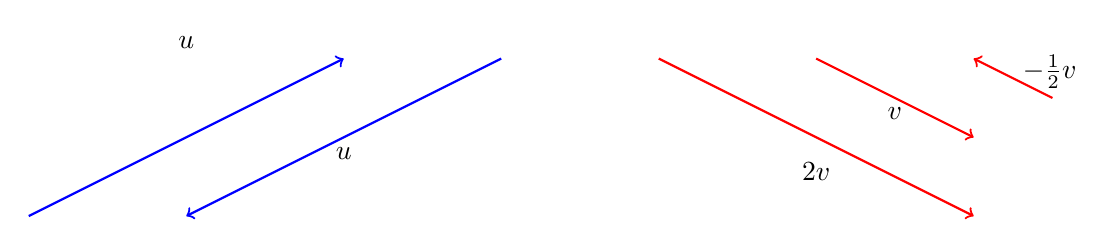
\begin{tikzpicture}[scale=2]
        \draw[->, thick, blue] (0,0)--(2,1);
        \draw[->, thick, blue] (3,1)--(1,0);
        \draw[->, thick, red] (5,1)--(6,0.5);
        \draw[->, thick, red] (6.5,0.75)--(6,1);
        \draw[->, thick, red] (4,1)--(6,0);
        \node[above] at (1,1){$\vect{u}$};
        \node[below] at (2,0.5){$\vect{u}$};
        \node[below] at (5.5, 0.75){$\vect{v}$};
        \node[above right] at (6.25, 0.75){$-\frac{1}{2}\vect{v}$};
        \node[below] at (5, 0.4){$2\vect{v}$};
      \end{tikzpicture}
    \end{center}
  \end{sol}
\end{ex}

\begin{ex}
  Find $-3\begin{mymatrix}{r}
    5 \\
    -1 \\
    2 \\
    -3
  \end{mymatrix} +5\begin{mymatrix}{r}
    -8 \\
    2 \\
    -3 \\
    6
  \end{mymatrix}$.
  \begin{sol}
    $\begin{mymatrix}{r}
      -55 \\
      13 \\
      -21 \\
      39
    \end{mymatrix}$.
  \end{sol}
\end{ex}

\begin{ex}
  Use the properties of scalar multiplication from
  Theorem~\ref{thm:vector-scalar-multiplication} and the properties of vector
  addition from Theorem~\ref{thm:properties-vector-addition} to prove
  the following equalities. Justify every step.
  \begin{enumerate}
  \item $(k+\ell)(\vect{u}+\vect{v}) = k\vect{u} + k\vect{v} +
    \ell\vect{u} + \ell\vect{v}$.
  \item $0\vect{u} = \vect{0}$.
  \item $(-1)\vect{u} = -\vect{u}$.
  \item $-(k\vect{u}) = k(-\vect{u}) = (-k)\vect{u}$.
  \end{enumerate}
  \begin{sol}
    \begin{enumerate}
    \item
      $(k+\ell)(\vect{u}+\vect{v}) = (k+\ell)\vect{u} +
      (k+\ell)\vect{v} = k\vect{u} + k\vect{v} + \ell\vect{u} +
      \ell\vect{v}$. Here we used the distributive law over vector
      addition in the first step, and the distributive law over scalar
      addition in the second step.
    \item We have $0\vect{u} = (0+0)\vect{u} = 0\vect{u} + 0\vect{u}$
      by properties of scalars and by the distributive law,
      respectively. Adding $-(0\vect{u})$ to both sides of the
      equation, and using the additive unit law and associativity, we
      have $\vect{0} = 0\vect{u}$.
    \item We have $(-1)\vect{u} = (-1)\vect{u} + \vect{0} =
      (-1)\vect{u} + (\vect{u} + (-\vect{u}) = ((-1)\vect{u} +
      \vect{u}) + (-\vect{u}) = ((-1)\vect{u} + 1\vect{u}) +
      (-\vect{u}) = ((-1)+1)\vect{u} + (-\vect{u}) = 0\vect{u} +
      (-\vect{u}) = \vect{0} + (-\vect{u}) = -\vect{u}$. Here, we have
      used the additive unit law, the additive inverse law, the
      associative law, the rule for multiplication by 1, the
      distributive law, properties of scalars, the property of part
      (b), and the additive unit law, respectively.
    \end{enumerate}
  \end{sol}
\end{ex}

